% Nicholas Arnold
% Steven Braeger
% COP 6616
%
% Project Progress Report
%
% We used the template from IEEE website, linked from
% http://www.ieee.org/conferences_events/conferences/publishing/templates.html	

\documentclass[conference]{IEEEtran}
\usepackage{algorithm}
\usepackage{algorithmic}

% *** CITATION PACKAGES ***
%
%\usepackage{cite}
% cite.sty was written by Donald Arseneau
% V1.6 and later of IEEEtran pre-defines the format of the cite.sty package
% \cite{} output to follow that of IEEE. Loading the cite package will
% result in citation numbers being automatically sorted and properly
% "compressed/ranged". e.g., [1], [9], [2], [7], [5], [6] without using
% cite.sty will become [1], [2], [5]--[7], [9] using cite.sty. cite.sty's
% \cite will automatically add leading space, if needed. Use cite.sty's
% noadjust option (cite.sty V3.8 and later) if you want to turn this off.
% cite.sty is already installed on most LaTeX systems. Be sure and use
% version 4.0 (2003-05-27) and later if using hyperref.sty. cite.sty does
% not currently provide for hyperlinked citations.
% The latest version can be obtained at:
% http://www.ctan.org/tex-archive/macros/latex/contrib/cite/
% The documentation is contained in the cite.sty file itself.

% *** MATH PACKAGES ***
%
%\usepackage[cmex10]{amsmath}
% *** SPECIALIZED LIST PACKAGES ***
%
%\usepackage{algorithmic}
% algorithmic.sty was written by Peter Williams and Rogerio Brito.
% This package provides an algorithmic environment fo describing algorithms.
% You can use the algorithmic environment in-text or within a figure


% *** ALIGNMENT PACKAGES ***
%
%\usepackage{array}
%\usepackage{mdwmath}
%\usepackage{mdwtab}
%\usepackage{eqparbox}

% *** SUBFIGURE PACKAGES ***
%\usepackage[tight,footnotesize]{subfigure}

%\usepackage[caption=false]{caption}
%\usepackage[font=footnotesize]{subfig}
%\usepackage{fixltx2e}
%\usepackage{stfloats}
% stfloats.sty was written by Sigitas Tolusis. This package gives LaTeX2e
% the ability to do double column floats at the bottom of the page as well
% as the top. (e.g., "\begin{figure*}[!b]" is not normally possible in
% LaTeX2e). It also provides a command:
%\fnbelowfloat
% to enable the placement of footnotes below bottom floats (the standard
% LaTeX2e kernel puts them above bottom floats). This is an invasive package

% Other Packages
\usepackage{moreverb}
\usepackage{graphicx}
\usepackage{caption}
\usepackage{url}

% correct bad hyphenation here
\hyphenation{op-tical net-works semi-conduc-tor}


\begin{document}
%
% paper title
% can use linebreaks \\ within to get better formatting as desired
\title{Scalable N-Body Event Prediction}


% author names and affiliations
% use a multiple column layout for up to three different
% affiliations
\author{\IEEEauthorblockN{Steven Braeger}
\IEEEauthorblockA{Department of Electrical Engineering and\\Computer Science\\
University of Central Florida\\
Orlando, Florida 32826\\
Email: \texttt{steve@soapforge.com}}
\and\IEEEauthorblockN{Nicholas Arnold}
\IEEEauthorblockA{Department of Electrical Engineering and\\Computer Science\\
University of Central Florida\\
Orlando, Florida 32826\\
Email: \texttt{narnold@knights.ucf.edu}}
}

\maketitle


\begin{abstract} %Steven
The general simulation of n-body systems often requires the simulation of pairwise interaction events between the objects.  The naive method of simulating these events is an algorithm that polls each pair of object for an interaction every timestep.  This algorithm has $O(n^2)$ operations per timestep in the number of objects.  However, this method scales very well to multiple cores. In this paper, we propose a novel method of pairwise simulation that saves a significant amount of computation time by predicting possible future outcomes rather than reacting to them.  We demonstrate the implementation of this method, as well as prove that it has amortized $O(n)$ complexity per timestep.  We also demonstrate a lock-free implementation to allow this algorithm to scale comparably to multiple cores of a shared memory machine.
\end{abstract}

\IEEEpeerreviewmaketitle


\section{Introduction}

There is a great deal of interest in discrete event simulation as it applies to video games and real time simulation. One interest in particular is the application of realistic physics in these simulations.  This kind of discrete event simulation is traditionally performed on large scale parallel clusters for film and scientific applications, or on massively parallel GPU architectures \cite{grape,uberflow}.  Specifically, we wish to explore the simulation and evolution of systems of dynamic and static objects where all the dynamic objects interact with all of the other objects, as happens when the dynamic objects physically collide with other objects.  In order to do this, we need to be able to model and react to collisions and interactions between objects. 

Although the naive and semi-naive implementations of this kind of simulation are embarassingly parallel, they are also exceedingly wasteful.  The method used to evaluate the interactions between objects is similar to a busy-wait loop, where all objects are continually polled, waiting for collisions to occur as the simulation progresses \cite{nbodycollisions,Moore88collisiondetection}.   As we will describe in the next sections, we are interested in using a novel predictive model along with a novel lock-free n-body event queue data structure to attempt to make a new kind of economical collision simulation system.  Our hope is that this system does not perform wasteful checks when checks are unlikely and maintains much of the parallelism of the naive solution.

\section{Problem Definition}

As input, we are given a description of static objects, dynamic objects, and the geometry defining their boundaries.  We are also given initial states like position, acceleration and velocity of the objects in the system, and a set of rules to update those objects.  As output, we wish to compute the exact state of each object in the system for each of the $n$ timestamps $t_0, t_1, t_2, \ldots, t_n$.

For each object $o$ in the system, a subroutine is defined \texttt{update($o$,$dt$)}, which computes the state of the object in the next timestamp, given the object state in the current timestamp and a time $dt$ between timestamps.  For each pair of objects $o1$ and $o2$, an additional subroutine is defined \texttt{collide($o1$,$o2$)} which computes the state of both $o1$ and $o2$ in the next timestamp, assuming that the objects have collided during the current timestamp.

\subsection{Naive Algorithm}

The brute force all-pairs solution is the naive solution to this problem as it is commonly implemented in games. This technique is known as a 'detection' technique because it relies on the idea of detecting a collision when it occurs instead of predicting a collision.  

\begin{algorithm}
\caption{Naive Algorithm}
\begin{algorithmic}
\FOR{each timestep $ti$}
	\FOR{each dynamic object $do$}
		\STATE update($do,dt$)  \COMMENT{$dt$ is the constant timestep difference}
		\FOR{each object $o$}
			\IF{check($do, o$)}
				\STATE collide($do, o, dt$)
			\ENDIF
		\ENDFOR
	\ENDFOR
\ENDFOR
\end{algorithmic}
\end{algorithm}

This technique is embarassingly parallel, allowing a thread per dynamic object or even a thread per pair with minimal overhead.  However, it is extremely
wasteful, because there are $O(n^2)$ checks being made every single timestamp, even if the likelihood of a collision has changed little since the last timestep \cite{Seningood}.  

Each of these $O(n^2)$ checks per timestep is computationally cheap individually, but when the number of objects is very great the computational overhead of performing all of them becomes
unmanagable. Considering that an extreme majority of the checks will fail due to the fact that collision occurrances are rare, most of them do not need to be computed, and avoiding their computation has the ability to dramatically increase the 
throughput of our simulation.

\subsection{Semi-Naive Algorithm}

A similar algorithm that we refer to as the 'semi-naive' algorithm has also found great use in practical applications \cite{Bittner02hierarchicaltechniques}.  The semi-naive algorithm differs only from the naive algorithm in that it exploits a bounding volume hierarchy to spatially partition the dynamic objects and pre-filter the collision checks.  This algorithm is equally wasteful, but only has $O(n log n)$ checks if the objects are relatively equally distributed throughout the bounding space.

\section{Theoretical Contribution}
\label{sec:theocont}
\subsection{Predictive Algorithm}

In our desired solution, we take a completely different approach.  In contrast to the naive and semi-naive algorithms, our solution avoids computing any unneeded checks on timestamps that do not change the solution by \textit{predicting} the intersections before they occur, rather than checking for them when they do not.  Our algorithm will use a slightly more complex subroutine \texttt{predict($o1$,$o2$)} that returns the time an intersection is likely to occur, and enters it into an event queue that contains the predicted collisions that are likely to occur.  When an intersection occurs, it is recomputed and removed from the queue.

\begin{algorithm}
\caption{Predictive Algorithm}
\begin{algorithmic}
\STATE \COMMENT{initialize events from initial states} % future_event_queue()
\FOR{each timestep $ti$}
	\FOR{each dynamic object $do$}
		\STATE update($do,dt$)  \COMMENT{$dt$ is the constant timestep difference}
		\STATE \COMMENT{for each event that occurs in this timestep}
		\FOR{each e in events.find(ti)}
			\FOR{each object $o$}
				\IF{check($e.o,o$)}
					\STATE collide($e.o, o, dt$) \COMMENT{predict next collision event into queue}
				\ENDIF
			\ENDFOR
			\STATE{$events$.remove($e$)}
		\ENDFOR
	\ENDFOR
\ENDFOR
\RETURN events
\end{algorithmic}
\end{algorithm}

It is worth noting that although our solution is the same runtime complextiy as the naive solution in the worst case (and, in fact, the initial population of event queue will need to preform $n^2$ predictions), it is unlikely to compute ANY checks that are unlikely to occur, thus saving tremendous computation time.  

However, our work is not done.  This algorithm is difficult to parallelize when compared to the naive algorithm, as it depends implicitly on reading and writing the global future nbody event queue data structure described in section \ref{sec:neq}.  This data structure is a specialized queue in which events take priority over other events about to take place. If we split the evaluation of the simulation into threads, then each thread must somehow synchronize which events it will prioritize and avoid collisions.  Furthermore, threads must be able to communicate and respond to future events  globally as collisions are predicted into the future.  This communication overhead is difficult to parallelize correctly, and will be the focus of our research.

\subsection{N-Body Future Event Queue}
\label{sec:neq}
Our algorithm depends on a data structure we call an "N-Body Future Event Queue".  This data structure is designed to facilitate the prediction algorithm
by storing pairwise events that are probabilistically likely (but not guaranteed) to occur.  Such a data structure has the following pseudocode description
\floatname{algorithm}{Data Structure}
\begin{algorithm}
\caption{Future Event Queue}
\begin{algorithmic}
\STATE \COMMENT{inserts an event into the queue, possibly superceding any events that happen later}
\STATE \textbf{insert}($event$)
\STATE \COMMENT{removes an event from the queue}
\STATE \textbf{remove}($event$)
	
\STATE \COMMENT{returns an iterator that iterates over all predicted events that occur after time $t$}
\STATE EventIterator \textbf{find}(time $t$)

\STATE \COMMENT{Returns all objects for which nothing is known about their behavior}
\STATE ObjectIterator \textbf{find\_invalid}()
\end{algorithmic}
\end{algorithm}

It is important to take special note here of the operations in the future event queue.  The most important differences from it and a standard priority queue or event queue
is that the find() method can search for all events that occur within a certain timeframe, and that events that get input into the queue are not necessarily persistent, as they 
may be superceded by events that are inserted later but are queued to occur before.  An event A in the queue supercedes an event B iff event A and B have an object in common AND A is scheduled to occur BEFORE B.

Lastly, ``find invalid'' is important because it is assumed that at some point some event will occur to all objects, otherwise simulating them is 
useless.  Thus, any objects which are in the scene but not present in the future event queue would indicate an error in our simulation logic.  In our example, even objects which
will not collide with any other objects must eventually collide with the boundaries of the simulation volume.  If no such collisions were known about
an object, we must know of this immediately and attempt to repredict that object's future.

In addition, our queue must implement these algorithms efficiently in order to get the desired average-case $O(n)$ performance that is an improvement over our prediction algorithm.  In particular, all operations must be implemented in $O(n)$ time.

\section{Scalable Implementation}
In this section, we propose a scalable lock-free implementation of the predictive algorithm from section \ref{sec:theocont}, including an implementation of the 
N-Body Future Event Queue data structure.  Our implementation uses barriers and hardware atomic compare-and-swap primatives to guarantee thread-safety.  Our scalable implementation
works in two parts, which we will discuss here:  First, it uses barriers and an hardware compare-and-exchange boolean to synchronize the algorithm that utilizes the data structure, 
a process that is described in Section \ref{sec:stsp}.  Next, it uses an array with a thread-safe indexing scheme to implement the future event queue which is described in Section \ref{sec:feq}
\subsection{Barriers}
\label{sec:barrier}
A barrier is a construct that is crucial to any threaded simulation.  It is a simple synchronization primative that only has one operation: wait(n).  
A thread that enters wait(n) will wait at that point in the control flow of the program until the total number of threads in the wait(n) function is n.  Then,
all threads return simultaneously.

Typically, a barrier is not classified as a lock-free operation.  In most implementations of a barrier, a locked mutex is used to sleep all the threads, which is 
unlocked when the number of sleeping threads is equal to n.  However, this need not be the case.  We observe that the barrier preserves the lock-free property if it is implemented
using a hardware atomic instructions instead.  Wait can be implemented as 

\floatname{algorithm}{Procedure}
\begin{algorithm}
\label{barrier}
\caption{Wait}
\begin{algorithmic}
\STATE barrier
	\STATE int $num\_threads$ \COMMENT{the number of threads to collect}
	\STATE wait()
	\STATE \COMMENT{collect this thread}
	\STATE fetch\_and\_sub($\&num_threads$,1)
	\STATE \COMMENT{spin until all threads are collected}
	\WHILE {$num\_threads > 0$}
		\STATE \COMMENT{uncollect this thread}
		\STATE fetch\_and\_add($\&num_threads$, 1)
	\ENDWHILE
\end{algorithmic}
\end{algorithm}

When implemented in this way, the implementation preserves the lock-free property, because even though n-1 threads are forced to wait, the last thread never waits for any 
mutex, or does it ever enter the spinlock loop.  The last thread does useful work until it enters the wait() body, then immediately exits, continuing to make progress, releasing all
other threads in the process.

\subsection{Scalable Timestep Sub-Phases}
\label{sec:stsp}
In all threaded implementations of timestamp-based simulation, at least one barrier construct
is necessary in order to prevent the system from processing more than one timestep at a time.  Without an implict barrier at the beginning or end of the 
processing for each timestamp, then worker threads could easily get out of sync on the timesteps that they are working on, which would produce incorrect calculations
for comparisons between threads.  The current timestamp of the simulation must be constant across all threads, and so a barrier is used in order to synchronize that timestamp.  This
limitation is true for all threaded timestep simulation, our application included.

Therefore, we can consider the timespan of a single timestep as a single computational unit, the beginning and end of which all threads are operating in sync.  We can ignore
all processing that occurs outside of a single timestep.  For our implementation of the prediction algorithm described in \ref{sec:theocont}, a single timestep is broken down
into several distinct 'phases`., with the overall structure as follows:

\floatname{algorithm}{Procedure}
\begin{algorithm}
\caption{Timestep}
\begin{algorithmic}
\STATE check\_react\_collisions();
\STATE repredict();
\STATE update\_simulation();
\STATE timestep\_sync\_barrier.wait();
\end{algorithmic}
\end{algorithm}

Note the implicit barrier protecting all threads from moving to the next frame before their peers.  The implementations of each subroutine are given in section \ref{sec:subphase}.

The primary problem with thread safety in this formulation of the timestep is the program errors that can occur in the status of the queue and the determinism of the simulation
if multiple threads are in different phases simultaneously.  For example, if thread A is updating object j, in the ``update simulation stage'', and thread B is writing to object 
j and i in the ``check react collisions'' phase, then the exact results the simulation will calculate are non-deterministic based on processor scheduling.  
Due to the fact that there are 3 phases, and $n$ objects, the total number of possible non-deterministic phase-overlap outcomes is $3x3xn=9n$.  This is clearly not an thread-safe solution.

However, as can be seen from section \ref{sec:subphase}, each of the subphases can be parallelized somewhat trivially.  Additionally, each subphase either reads and writes
a single array for that phase without inter-thread communication, or reads and writes two arrays with inter-thread communication.  Therefore, to allow us to parallize each
phase in isolation, we break up the timestep into ``sub-phases'' using an additional barrier operation, implemented as in section \ref{sec:barrier}.  

\floatname{algorithm}{Procedure}
\begin{algorithm}
\caption{Check\_React\_Collisions}
\begin{algorithmic}
\STATE \COMMENT{search event queue for events that are occuring now}
\FOR{$e$ in $events$.find($current\_time$)}
	\STATE \COMMENT{if the event happens}
	\IF{check($e.o1,e.o2$)}
		\STATE \COMMENT{modify both objects}
		\STATE collide($e.o1,e.o2$)
	\ENDIF
	\STATE \COMMENT{the event is passed, so remove it.}
	\STATE $events$.remove($e$)
\ENDFOR
\end{algorithmic}
\end{algorithm}

This way, we can guarantee that each thread never has cross-phase non-determinism, reducing the number of potential non-deterministic concurrency cases to account for from $9n to 3n$
Furthermore, as we will demonstrate, the update phase and the repredict phase are embarassingly parallel and require no cross-thread communication or synchronization,
reducing the synchronization concerns to only the implementation of check-react.

\subsection{Lock-Free Subphases}
\label{sec:subphase}
\subsubsection{Update}

The update phase is simple and embarasingly parallel.  It also demonstrates our overall technique to distribute work equally to multiple threads.  In most of our sub-phases,
we evenly distribute one object to perform operations on to each thread, evenly, one at a time by using a hash function that maps object ids to thread ids evenly. $thread(object\_id) = object\_id \% num\_threads + thread\_id$
\floatname{algorithm}{Procedure}
\begin{algorithm}
\caption{Update\_Simulation}
\begin{algorithmic}
\FOR {every object $o$ assigned to $current\_thread$}
	\STATE update($o$)
\ENDFOR
\end{algorithmic}
\end{algorithm}

Because updating an object only modifies that particular object, this phase is embarrassingly data-parallel and needs no additional synchronization.

\subsubsection{Check-React}

\floatname{algorithm}{Procedure}
\begin{algorithm}
\caption{Check\_React\_Collisions}
\begin{algorithmic}
\STATE \COMMENT{search event queue for events that are occuring now}
\FOR{$e$ in $events$.find($current\_time$)}
	\STATE \COMMENT{if the event happens and this thread is assigned to it}
	\IF{$e$.$o1$ is in $current\_thread$ and check($e.o1,e.o2$)}
		\STATE \COMMENT{modify both objects}
		\STATE collide($e.o1,e.o2$)
	\ENDIF
	\STATE \COMMENT{the event is passed, so remove it.}
	\STATE $events$.remove($e$)
\ENDFOR
\end{algorithmic}
\end{algorithm}
This phase does the grunt work of the predictive algorithm.  During this phase, pending events that were predicted to happen in the current timestep are checked to see if they actually occur.  This phase requires additional synchronization overhead for several reasons.

\begin{enumerate}
	\item collide() reads and writes TWO objects, which means it could potentially modify objects that are assigned to other threads non-deterministically.
	\item There could be two events in the queue which actually describe the same event but swap the order of the objects, which could mean that a collide() reaction to the event could be triggered twice in the same frame.
	\item Multiple threads could check() an object while another object is in the middle of writing to it.
\end{enumerate}

However, we can exploit the structure of our problem in order to guarantee that none of these cases occur.  Due to the fact that for two symmetric events, we only want one... we can check to see if one or both of the objects in the set have already been collided.
We can do this by using a flag bit for each of the objects in the scene to check whether or not the objects have been collided yet this frame.  Then, we check
that bit for the OTHER object in our comparison, to see if the collision has already occured.  Regardless of whether or not the bit is set, we wish to atomically
update the status of that bit to true for our current object.  The code becomes as follows.

\floatname{algorithm}{Procedure}
\begin{algorithm}
\caption{Check\_React\_Collisions}
\begin{algorithmic}
\STATE \COMMENT{search event queue for events that are occuring now}
\FOR{$e$ in $events$.find($current\_time$)}
	\STATE \COMMENT{if object reacted yet is false,set reacted to true and do the event}
	\IF{!compare\_and\_exchange(reacted\_yet[$e.o1$],false,true)}
		\STATE \COMMENT{if the event hasn't been  happens and this thread is assigned to it}
		\IF{$e.o1$ is in current\_thread and check($e.o1,e.o2$)}
			\STATE \COMMENT{modify both objects}
			\STATE collide($e.o1,e.o2$)
		\ENDIF
		\STATE \COMMENT{the event is passed, so remove it.}
		\STATE $events$.remove($e$)
	\ENDIF
\ENDFOR
\end{algorithmic}
\end{algorithm}


\subsubsection{Repredict}
\label{sec:repredict}
The reprediction phase is slightly more complex, but it is also embarassingly parallel and lock-free, provided that the implementation of our future event queue is thread-safe and scalable as well.  It detects simulation errors of the sort described in section \ref{sec:neq}, and also re-predicts collisions
that have been removed in check-react.  After finding all of the invalid objects (objects with no known future) that have been recently invalidated by check-react as well as logic errors, it then
searches for all known predictions that will occur in the future and puts them into the queue.  
\begin{algorithm}
\caption{Repredict()}
\begin{algorithmic}
\STATE \COMMENT{search event queue for objects that the queue is unaware of}
\FOR{$oinvalid$ in $events$.find\_invalid($current\_time$)}
	\STATE \COMMENT{if invalid object is assigned to this thread}
        \IF{$oinvalid$ in current\_thread}
		\FORALL{dynamic\_objects $do$}
			\STATE $events$.insert(predict($oinvalid,do$))
		\ENDFOR
	\ENDIF
\ENDFOR
\end{algorithmic}
\end{algorithm}
This algorithm is thread-safe and lock-free provided that the implementations of events.insert and events.find\_invalid are thread-safe and lock-free, because predict is a read-only method that 
does not write to non-thread assigned data, even though it reads the current state of all dynamic objects in the scene.

In the case of an empty future queue, this phase is $O(n^2)$, because it has to make predictions on all pairs of objects.  However, in order for that to occur in the average case would require a majority of frames to have all objects collide
with some other object simultaneously, a case which is exceedingly rare for the simulations we wish to run.

\subsection{Future Event Queue}
\label{feq}
The future event queue stores N-body events, and is designed to be used in concert with the sub-phase algorithm as described in Section \ref{sec:subphase}.
Our implementation uses an array to store a series of one-element priority-queues: one for each object in the scene.  This array shows the current best-guess
prediction of events that are inbound on the object.  The advantage of this approach is that our predictive queue doesn't have to deal with the contention of 
a standard queue implemented in a list, and it is also space efficient, as it is able to throw away events that supercede other events at insertion time.


\subsubsection{insert}

The implementation of insert is protected by the fact that an event that is inserted containing object $i$ as the first object in the event will only
be inserted from the thread that owns object $i$, as can be seen from section \ref{sec:repredict}.  Thus, insert requires no synchronization, as it can be verified
that no other thread will read or write to this same location during the react subphase.  It is important to note that this implementation can and does remove events,
and would not be suitable for any other kind of event queue.  However, our application domain says that removing potential events that will not occur from the queue is a feature, not a bug.

\begin{verbatimtab}[3]
FutureEventQueue::insert(event e)
{
   if(!this.current_events[e.o1].valid OR this.current_events.time > e.time)
	this.current_events[e.o1]=e;
}
\end{verbatimtab}

This definition of insert runs in $O(1)$ time, which is actually much better then our requirement that it runs in $O(n)$ time.

\subsubsection{remove}

Remove is similar to insert, except it simply sets the event to invalid in the array queue.  It too is $O(1)$

\begin{verbatimtab}[3]
FutureEventQueue::remove(event e)
{
	this.current_events[e.o1].invalid;
}
\end{verbatimtab}

\subsubsection{find\_invalid}

The implementation of find\_invalid with our array-based queue is simply a linear search for any events that are marked as invalid in the array.
However, because of our previous rule that the event array cannot be read or written by a thread not its owner in the same phase, we only return invalid
objects from the objects in the current thread.  Although this would seem to break the functionality of find\_invalid, this behavior simply serves to reinforce
the constraint given in \ref{sec:repredict} that threads can only repredict objects they own. It also meas that we never repredict objects across thread
ownership boundaries.

\begin{verbatimtab}[3]
ObjectIterator FutureEventQueue::find_invalid()
{
   for o in dynamic_objects
   {
      if(o in current_thread AND !this.current_events[o].valid)
      {
      #return object as part of invalid set for this thread.
	yield o;
      }
   }
}
\end{verbatimtab}

Find invalid runs in $O(n)$ space and time.

\subsubsection{find}

Similar to the implementation of find\_invalid, the implementation of find also is implemented based on a linear search.  It finds all valid events
and also checks to make sure that those events are happening in the current frame.

\begin{verbatimtab}[3]
EventIterator FutureEventQueue::find(current_time)
{
   for o in dynamic_objects
   {
      if(o in current_thread AND this.current_events[o].valid AND this.current_events[o].time <= current_time)
      #return the event that is about to occur
	yield this.current_events[o];
   }
}
\end{verbatimtab}

\subsection{Summary of Predictive Method}
	The subphase barriers and the thread object ownership system work together to ensure the thread-safety of the inputs and outputs to the Future Event Queue.
This partnership ensures in all the covered cases that the same object data is never used as a concurrent shared resource for both reading and writing.  In addition, we believe our algorithm maintains
the lock-free property because it remains wait-free in all states except when a thread is waiting at a barrier, which we justified is still a lock-free state in Section \ref{barrier}.

\section{Experimental Setup}%Nick

In order to test our algorithm, we implemented a particular instance of future event simulation in the detection of collisions between two objects.

In typical instances of this problem in the real world, the type of simulation varies dramatically. In many applications, the objects obey complex interaction patterns such as flocking behavior and user interaction.  However, these interactions are almost always built around a simple framework for simulation that obeys Newtonian physics as the primary motion characteristic, with the more complex
behaviors simply activating different Newtonian trajectories and velocities \cite{Jadbabaie02coordinationof}.  Therefore, without loss of generality, we will simplifiy our simulation by limiting the object behaviors to simulate Newtonian physical interactions of objects under Earth-like gravity.

For our simulation, since we are using dynamic spheres, we use the following calculations for the collision reaction\cite{wheatchex}:

\begin{math}
c = n \cdot (v_{1i} - v_{2i})
\end{math}

\begin{math}
v_{1f} = v_{1i} - \frac{m_2 \cdot c}{m_1 + m_2} \cdot (1 + e)n
\end{math}

\begin{math}
v_{2f} = v_{2i} + \frac{m_1 \cdot c}{m_1 + m_2} \cdot (1 + e)n
\end{math}

where:

$v_{1i}$ = the initial velocity of object 1

$v_{2i}$ = the initial velocity of object 2

$m_1$ = the mass of object 1

$m_2$ = the mass of object 2

$e$ = the coefficient of restitution ($e$ = 1 for completely elastic)

$n$ = normal unit vector drawn from object 1 to object 2


Real simulations may also involve extremely complicated geometry, such as the convex shapes of human faces, vehicles, and buildings.  However, 
all of these simulations generalize objects by a first pass of a 'bounding volume' for the more complex object.  The bounding volume is a simple shape (e.g., a sphere)
that forms a tight bounds on the object.  Real applications solve the first-pass collision checks for the simple 'bounding volume', and only fall back to a more complex
collision check on convex shapes if the bounding volumes intersect.  Thus, we can solve the problem without loss of generality by solving the problem
for simple bounding-volume shapes \cite{uberflow,cloth}.  In our case, we choose to use dynamic objects made of simple spheres, and static objects made of planes.

In order to program the simulation, we will use C++, as it is a good language for high performance simulation applications.  In order to facilitate our 
3D geometry and numerical libraries, we will write our own simulation system and geometry routines based on the C++ Numerical Vector library Eigen.  

We wish to test performance economy as well as parallizability.  For our parallization tests, we will use thread-level parallelism constructs from the C++11 standard and atomic primitives, if applicable.

The performance of these systems is typically evaluated in terms of a throughput measurement that measures the number of timestamps per second the system is capable of producing.  Equivalently, one can measure the average wall-clock time that passes while evaluating one timestamp.

\subsection{Naive Implementation}

The implementation of the naive solution is relatively straightforward, as a naive approach should be.  First, all of the dynamic objects must be updated for each timestamp to their new positions, using their previously calculated velocity vectors.  Then, because we are handling the spheres and planes separately, we have two sets of nested for loops to perform the collision checks.  The first loops over the spheres and checks each with all of the planes, and the second loops over the spheres and checks each with all of the spheres that are after it in the list.  We do this to avoid checking each pair twice (\texttt{collide($o1$,$o2$)} would evaluate the same as \texttt{collide($o2$,$o1$)}). For the threaded version of this algorithm, we parallel for loops:

\floatname{algorithm}{Algorithm}
\begin{algorithm}
\caption{Update}
\begin{algorithmic}
\FOR {$i = 0$ to $num\_spheres$}
	\STATE $dynamic_spheres$[$i$].update($dt$)
\ENDFOR
\end{algorithmic}
\end{algorithm}

\subsection{Predictive Implementation}

The scalable predictive implementation has aready been described in Section \ref{sec:theocont}.  However, we have not described the implementation of the sphere-sphere prediction algorithm.
This algorithm is relatively simple.  Given two spheres, we can describe their positions, accelerations, and velocities as the equation

\begin{equation}
   
\begin{verbatimtab}[3]
ObjectIterator FutureEventQueue::find_invalid()
{
   for o in dynamic_objects
   {
      if(o in current_thread AND !this.current_events[o].valid)
      #return object as part of invalid set for this thread.
	yield this.current_events[e.o1]=e;
   }
}
\end{verbatimtab}
\end{equation}


\section{Results} %Steven

The total runtime of the naive algorithm is scale-invariant.  That is to say it doesn't matter the size of the volume, the runtime is bound by the number of checks being performed, which is constant across varying volume sizes.  This scale-invariance is despite the reduction of actual collisions occurring volume size increases.  The total runtime shows polynomial growth due to the increasing number of collision checks as sphere count increases, which also shows polynomial growth.  Because of the vast number of collision checks occurring, prediction rates were between 0.0001\% and 0.05\% correct detection.

\begin{center}
	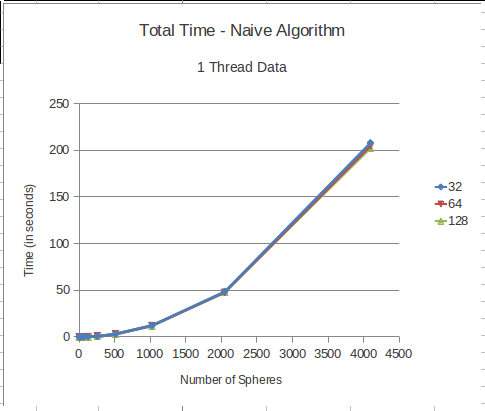
\includegraphics[width=.45\textwidth]{runtime_naive_1thread.png}
	\captionof{figure}{}
\end{center}

\begin{center}
	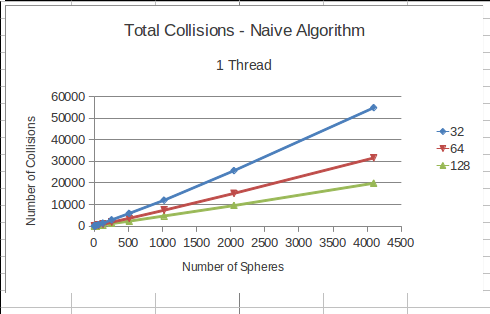
\includegraphics[width=.45\textwidth]{collisions_naive_1thread.png}
	\captionof{figure}{}
\end{center}

For the predictive algorithm, total runtime is not scale-invariant, as predictions rely on calculating physical collisons.  As the volume increases, the likelihood of collision decreases.  Total runtime is showing polynomial growth as was true with the naive algorithm, but at a much slower growth rate than the naive algorithm.  This may be a result of extra overhead to perform collision equation calculations in order to reduce the number of unnecessary collision checks.  The number of checks performed per timestep is linearly increasing, as opposed to the polynomial growth of the checks performed in the naive solution.  Prediction rates were between 0.3\% and 0.7\% correct, which although still low, are enormously more efficient when compared to the naive algorithm (see figure below).  These prediction rates are so low because at every timestep, the predictive algorithm still iterates over an array which holds future collision information.  Every array location maps to a sphere, and each location gets 'checked' once per timestep.  So an array location could be 'checked' many times before it actually triggers a collision event.

\begin{center}
	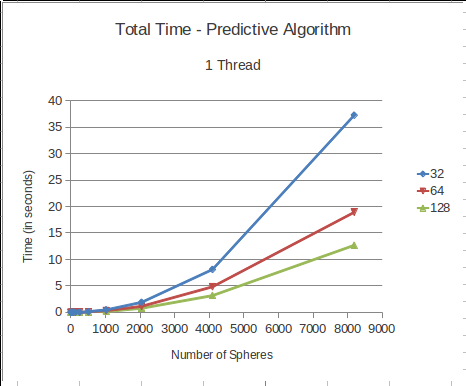
\includegraphics[width=.45\textwidth]{runtime_predictive_1thread.png}
	\captionof{figure}{}
\end{center}

\begin{center}
	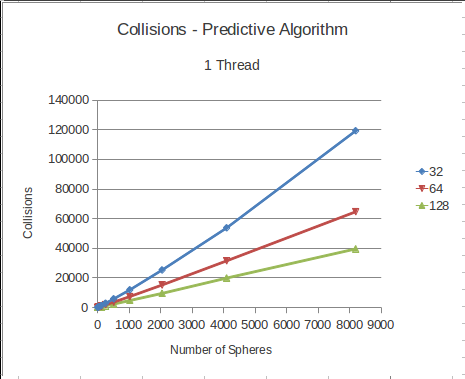
\includegraphics[width=.45\textwidth]{collisions_predictive_1thread.png}
	\captionof{figure}{}
\end{center}

\begin{center}
	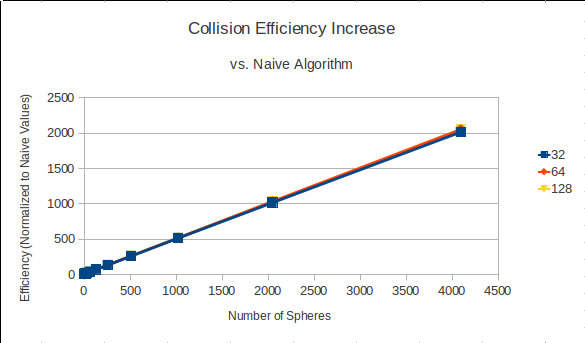
\includegraphics[width=.45\textwidth]{collision_efficiency.png}
	\captionof{figure}{}
\end{center}

When subjecting the naive solution to thread improvements, multiple threads offer faster run times as the number of spheres increases.  Total collisions detected are thread-invariant (as they should be), and scale linearly with the number of spheres in the scene.  Total checks are also thread-invariant (as they should be), and scale polynomially with the number of spheres in the scene.

\begin{center}
	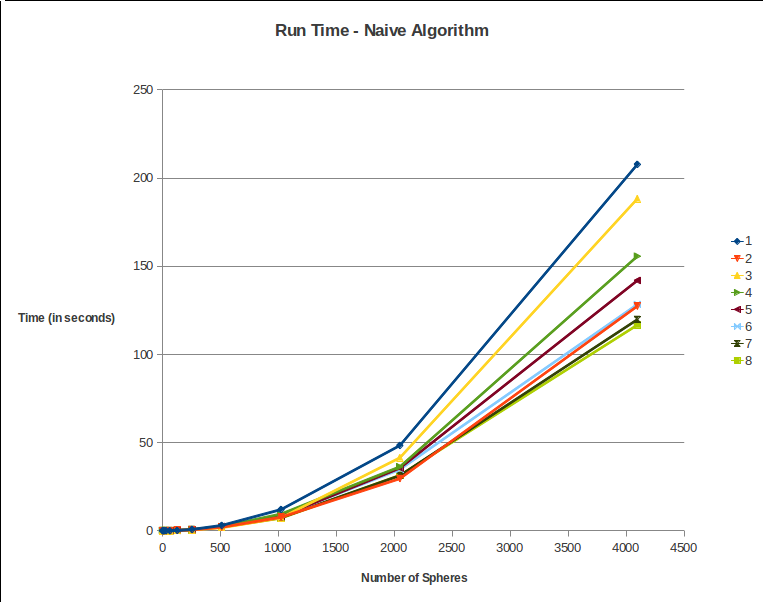
\includegraphics[width=.45\textwidth]{runtime_naive_allthreads.png}
	\captionof{figure}{}
\end{center}

\begin{center}
	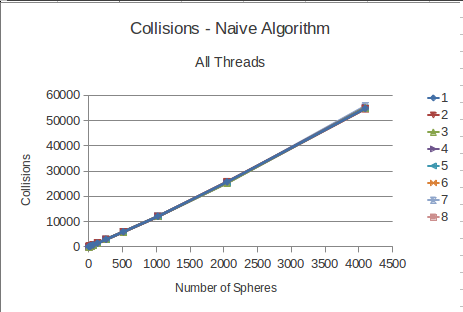
\includegraphics[width=.45\textwidth]{collisions_naive_allthreads.png}
	\captionof{figure}{}
\end{center}

Although single-threaded runs of the predictive algorithm show polynomial growth, it appears that multiple threads of the predictive algorithm begin to exhibit closer to linear growth.  As the number of spheres increases, the benefit of multiple threads increases as well.  Collisions and checks are also thread-invariant (as they should be), and with the predictive algorithm, both scale linearly with the number of spheres in the scene.

\begin{center}
	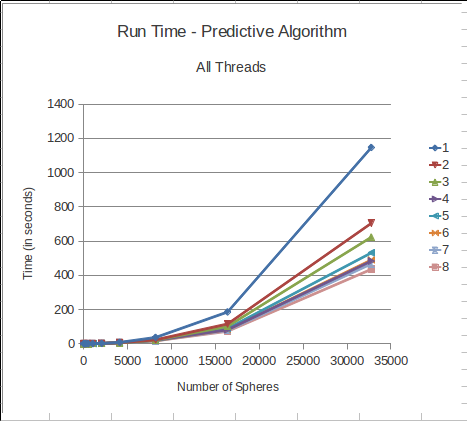
\includegraphics[width=.45\textwidth]{runtime_predictive_allthreads.png}
	\captionof{figure}{}
\end{center}

\begin{center}
	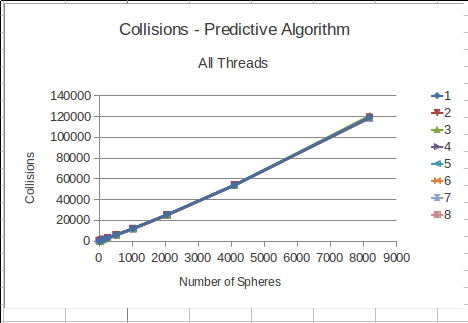
\includegraphics[width=.45\textwidth]{collisions_predictive_allthreads.png}
	\captionof{figure}{}
\end{center}

When comparing the runtimes of both algorithms and all thread scenarios, the predictive algorithm appears at this resolution to be linear with respect to the naive algorithm.  However, with the addition of a few extra simulations with even more spheres, we know this is not the case.  The runtimes do begin to exhibit a polynomial growth rate, albeit at a much slower growth.  For example, in our data, the predictive algorithm can handle four times as many spheres (shown by the 4096 naive spheres simulation runs just slightly longer than 16384 predictive spheres simulation) to execute in approximately the same runtime as the naive algorithm.

\begin{center}
	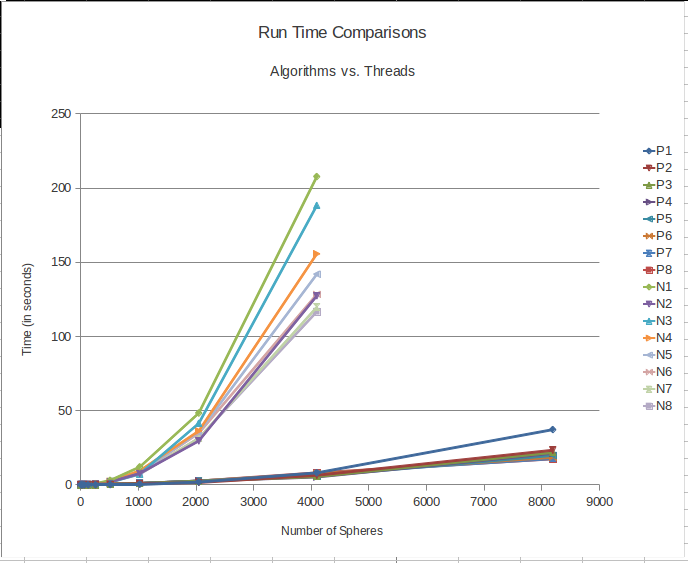
\includegraphics[width=.45\textwidth]{runtime_comparison.png}
	\captionof{figure}{}
\end{center}

With respect to the naive algorithm, the number of checks skyrocket quickly as the number of spheres increases.  In order to more easily visualize the magnitude of this increase, we have shown a log-log plot of the number of spheres for the simulation vs. the number of checks performed by each algorithm.  The plot shows that the number of checks performed in the naive algorithm quickly grow to at least 10 orders of magnitude (base 2) more than the predictive algorithm.

\begin{center}
	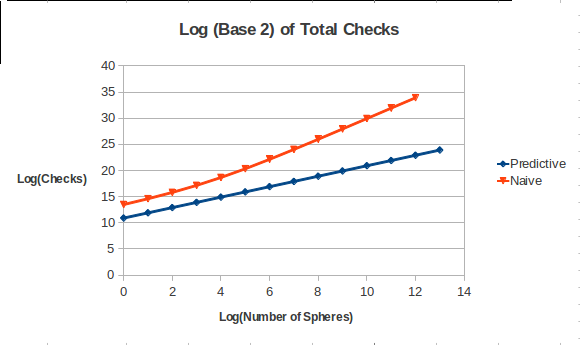
\includegraphics[width=.45\textwidth]{log_total_checks_comparison.png}
	\captionof{figure}{}
\end{center}

Next we show that both algorithms eventually gain a benefit from multithreading, in comparison with their single threaded counterparts.  In addition to the faster runtimes of the predictive algorithm, it also scales better than the naive solution as the number of spheres increases.  There is, however, a threshold on the predictive algorithm where there is no threading benefit (in our data, this threshold is between 2048 and 4096 spheres).  This could be caused by some kind of overhead in managing the threads that is a significant portion of the total runtime when there are very few spheres (the predictive algorithm runtime between 2048 and 4096 spheres is 2-8 seconds).  As the number of spheres increases, that overhead appears to become less and less dominant, and the performance improvement can be seen.  At 32768 spheres, the speedup with 8 threads is shown to be 2.6 times faster than the single threaded simulation.

\begin{center}
	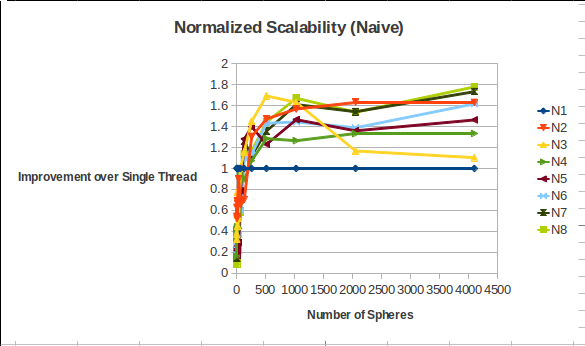
\includegraphics[width=.45\textwidth]{normalized_scalability_naive.png}
	\captionof{figure}{}
\end{center}

\begin{center}
	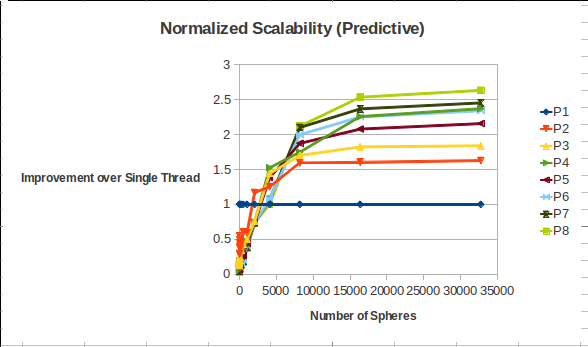
\includegraphics[width=.45\textwidth]{normalized_scalability_predictive.png}
	\captionof{figure}{}
\end{center}

\section{Conclusion} 


As we have only completed the preliminary set of data gathering, and have not implemented our predictive algorithm, we are not able to draw any conclusions as of yet.  Upon completion of the predictive algorithm implementation, and the subsequent data gathering and analysis, we will be able to form appropriate conclusions.

\bibliographystyle{IEEEtran}
\bibliography{IEEEabrv,midterm}

\appendix %Steven
\section{Project Progress}
This project is progressing well.  Save several hiccups in the implementation, we now have a very large and stable mature codebase that implements the naive implementations of the algorithm and allows
us to visualize the result.
\subsection{Challenges Encountered}
We encountered several challenges when implementing this project.  Although the simulation algorithm is simple in theory, debugging and implementing the physics behind the spheres caused a few small problems we did not foresee.

\subsubsection{Visualizer}
We had a great deal of small bugs that needed to be solved.  The primary method of solving this problem from a debugging perspective was the implementation of a real-time visualization in OpenGL.
This visualization was a little slow, but it facilitated debugging of our simulation.  Creating this visualization required some tweaking of the core simulator to allow a callback hook, as well as some OpenGL code to render the spheres in real-time.

\begin{center}
	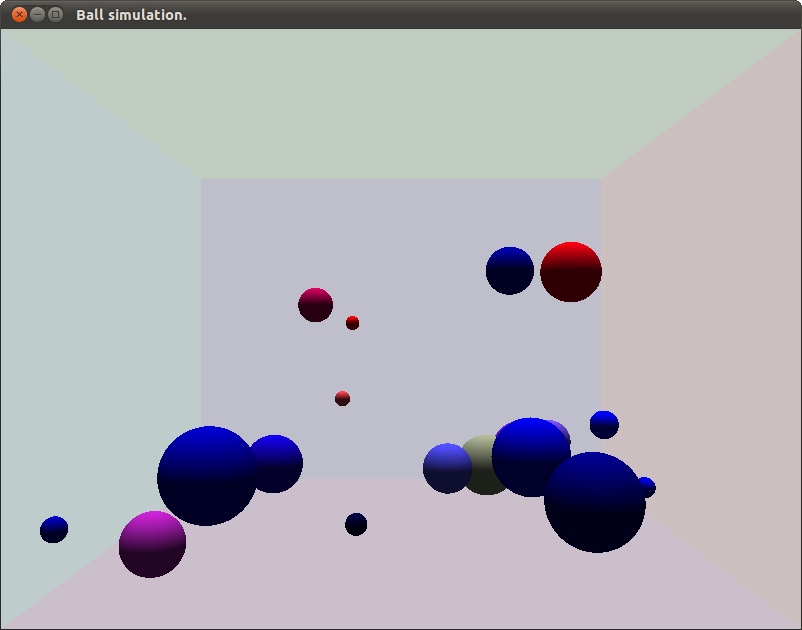
\includegraphics[width=.45\textwidth]{few.png}
	\captionof{figure}{A few balls}
	\label{fig:few}
\end{center}

\begin{center}
	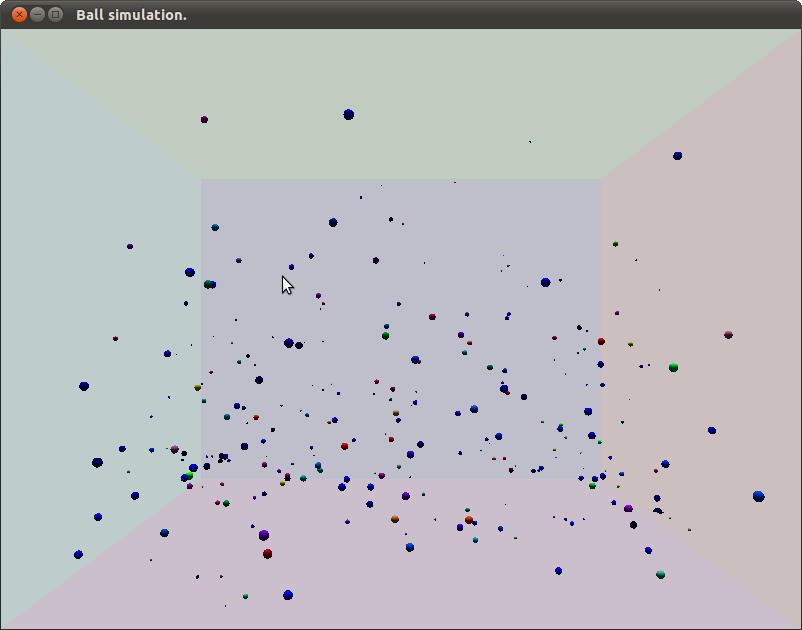
\includegraphics[width=.45\textwidth]{lots.png}
	\captionof{figure}{Lots of balls}
	\label{fig:lots}
\end{center}

\subsubsection{Sticky Spheres}
At our first running of the algorithm, we noticed that the number of registered sphere-sphere collisions was greater than the number of timesteps.  This should be impossible, as a sphere-sphere collision should
occur very rarely, depending on the total volume of the space and the number of spheres in the simulation.  Even when the number of spheres was 2, this phenomena occured.  Upon debugging the simulation with the visualizer,
we observed that any time a sphere collided with a larger sphere, it immediately became stuck inside the larger one, as shown in \ref{fig:linked}.  

\begin{center}
	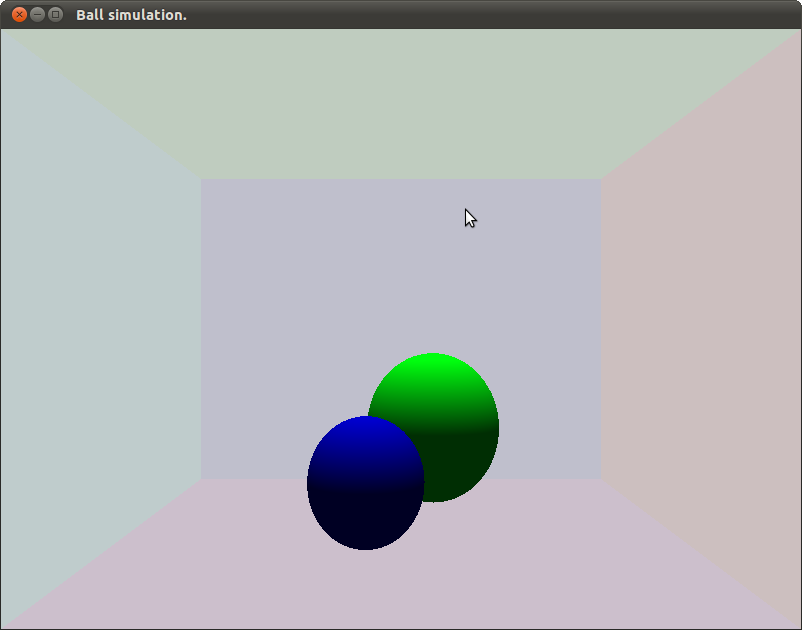
\includegraphics[width=.45\textwidth]{linked.png}
	\captionof{figure}{Two Linked Spheres}
	\label{fig:linked}
\end{center}

This problem generated 1 sphere-sphere collisions for each frame, for each pair of 'stuck' spheres.  To mitigate this problem, we implemented a simple hack that pushed the spheres away from each other by a distance equal to the sum of their radii plus an epsilon.
This dramatically reduced the number of sphere-sphere collisions to the correct number.

\subsubsection{Thread Overhead}
	Our implementation of the threading uses the OpenMP compiler extension subsystem.  Our implementation, which is a part of gcc 4.5, is built on top of pthreads under linux.  In our implementation, we 
spawn a number of worker threads per timestamp in order to thread the system.  Our implementation of the naive algorithm should scale linearly with the number of threads.  However, in our implementation this is not the case.  We strongly suspect that
several factors could be contributing to this difficulty.  

\begin{itemize}
	\item The overhead of spawning multiple threads per timestep dwarfs the work done by the update step
	\item The thread spawn behavior is sub-optimal as described by \cite{performance-critical}
	\item Thread affinity is poor.
	\item Threads may be competing for the global statistical variables we are using to measure performance.
\end{itemize}

We intend on investigating all of these possibilities immediately in the following weeks.  It is important to do so, because our argument for the applicability of this algorithm to parallel data-structures
is based on the necessity of competing with the highly-scalable naive algorithm.  If we fail to implement a scalable naive algorithm, then our ability to implement a scalable predictive algorithm is questionable.

\subsection{Completed Tasks}
\subsubsection{Simulation Framework}
We completed a simulation framework capable of interactively running our simulation in multiple different configurations from the command line.  Our simulation framework correctly
creates a simulation in a memory and cpu-efficiant way, and allows us to extend the implementation of the update step without changing the rest of the codebase.
\subsubsection{Visualization Framework}
In order to debug and to visualize the state of the simulation at a given timestep, a visualization in opengl was produced.
\subsubsection{Threaded and Non-Threaded Naive Implementation}
The implementation of our Naive algorithm is complete for the threaded and the non-threaded implementation.  However, as previously described, our implementation does not scale.  However, it is verified to function
correctly in both implementatons.

\subsection{Remaining Tasks}
There are 3 major tasks remaining.
\begin{itemize}
\item Fix the scalability of the naive algorithm and generate new data.
\item Write the predictive algorithm and test.
\item Finish the final report.
\end{itemize}

\subsection{Target Conference}
Currently, we would like to aim for a submission to the IEEE IPDPS Symposium (\url{http://ieeexplore.ieee.org/xpl/mostRecentIssue.jsp?punumber=5136864}).  In order to prepare for this submission, much additional research will be needed, with more detailed and robust follow up experimentation.  This experimentation will include, but not be limited to:
\begin{itemize}
\item implementation of the semi-naive algorithm,
\item robust and accurate physics calculations,
\item bug-free code base, and
\item more robust test cases.
\end{itemize}

% An example of a floating figure using the graphicx package.
% Note that \label must occur AFTER (or within) \caption.
% For figures, \caption should occur after the \includegraphics.
% Note that IEEEtran v1.7 and later has special internal code that
% is designed to preserve the operation of \label within \caption
% even when the captionsoff option is in effect. However, because
% of issues like this, it may be the safest practice to put all your
% \label just after \caption rather than within \caption{}.
%
% Reminder: the "draftcls" or "draftclsnofoot", not "draft", class
% option should be used if it is desired that the figures are to be
% displayed while in draft mode.
%
%\begin{figure}[!t]
%\centering
%\includegraphics[width=2.5in]{myfigure}
% where an .eps filename suffix will be assumed under latex, 
% and a .pdf suffix will be assumed for pdflatex; or what has been declared
% via \DeclareGraphicsExtensions.
%\caption{Simulation Results}
%\label{fig_sim}
%\end{figure}

% Note that IEEE typically puts floats only at the top, even when this
% results in a large percentage of a column being occupied by floats.


% An example of a double column floating figure using two subfigures.
% (The subfig.sty package must be loaded for this to work.)
% The subfigure \label commands are set within each subfloat command, the
% \label for the overall figure must come after \caption.
% \hfil must be used as a separator to get equal spacing.
% The subfigure.sty package works much the same way, except \subfigure is
% used instead of \subfloat.
%
%\begin{figure*}[!t]
%\centerline{\subfloat[Case I]\includegraphics[width=2.5in]{subfigcase1}%
%\label{fig_first_case}}
%\hfil
%\subfloat[Case II]{\includegraphics[width=2.5in]{subfigcase2}%
%\label{fig_second_case}}}
%\caption{Simulation results}
%\label{fig_sim}
%\end{figure*}
%
% Note that often IEEE papers with subfigures do not employ subfigure
% captions (using the optional argument to \subfloat), but instead will
% reference/describe all of them (a), (b), etc., within the main caption.


% An example of a floating table. Note that, for IEEE style tables, the 
% \caption command should come BEFORE the table. Table text will default to
% \footnotesize as IEEE normally uses this smaller font for tables.
% The \label must come after \caption as always.
%
%\begin{table}[!t]
%% increase table row spacing, adjust to taste
%\renewcommand{\arraystretch}{1.3}
% if using array.sty, it might be a good idea to tweak the value of
% \extrarowheight as needed to properly center the text within the cells
%\caption{An Example of a Table}
%\label{table_example}
%\centering
%% Some packages, such as MDW tools, offer better commands for making tables
%% than the plain LaTeX2e tabular which is used here.
%\begin{tabular}{|c||c|}
%\hline
%One & Two\\
%\hline
%Three & Four\\
%\hline
%\end{tabular}
%\end{table}


% Note that IEEE does not put floats in the very first column - or typically
% anywhere on the first page for that matter. Also, in-text middle ("here")
% positioning is not used. Most IEEE journals/conferences use top floats
% exclusively. Note that, LaTeX2e, unlike IEEE journals/conferences, places
% footnotes above bottom floats. This can be corrected via the \fnbelowfloat
% command of the stfloats package.


% trigger a \newpage just before the given reference
% number - used to balance the columns on the last page
% adjust value as needed - may need to be readjusted if
% the document is modified later
%\IEEEtriggeratref{8}
% The "triggered" command can be changed if desired:
%\IEEEtriggercmd{\enlargethispage{-5in}}

% references section

% can use a bibliography generated by BibTeX as a .bbl file
% BibTeX documentation can be easily obtained at:
% http://www.ctan.org/tex-archive/biblio/bibtex/contrib/doc/
% The IEEEtran BibTeX style support page is at:
% http://www.michaelshell.org/tex/ieeetran/bibtex/
%\bibliographystyle{IEEEtran}
% argument is your BibTeX string definitions and bibliography database(s)
%\bibliography{IEEEabrv,midterm.bib}
%
% <OR> manually copy in the resultant .bbl file
% set second argument of \begin to the number of references
% (used to reserve space for the reference number labels box)

%\begin{thebibliography}{1}

%\bibitem{IEEEhowto:kopka}
%H.~Kopka and P.~W. Daly, \emph{A Guide to \LaTeX}, 3rd~ed.\hskip 1em plus
%  0.5em minus 0.4em\relax Harlow, England: Addison-Wesley, 1999.

%\end{thebibliography}

%\bibliographystyle{ieeetr}
%\bibliography{midterm}

%\appendix
%\section{Project Progress}
%\subsection{Challenges Encountered}
%\subsection{Completed Tasks}
%\subsection{Remaining Tasks}


% that's all folks
%\bibliographystyle{ieeetr}
%\bibliography{midterm}




%\appendix
%\section{Project Progress}
%\subsection{Challenges Encountered}
%\subsection{Completed Tasks}
%\subsection{Remaining Tasks}

\end{document}


